% Grafikpaket laden
\usepackage{graphicx}
% hier beginnt das Dokument
\section{Hadoop}
\cite{Wartal2012}
\cite{Endlich2011}
\subsection{Einleitung}
Hadoop ist ein Java basiertes Open Source Framework von Apache. 
Die Entwicklung von Hadoop wurde als Teilpojekt von Nutch angefangen, welcher als die  Weiterentwicklung von Apache Lucene darstellte. Das Ziel des Projektes Nutch war eine schnelle Websuche, also eine Alternative zu Google. Die Herausforderung für die Nutch Entwickler war es ein System zu schaffen welches mit hoch skalierbaren Prozessen, Redundanzen, automatischen Fehlerbeseitigung und Verteilen der Last umgehen kann.  Als Google im Jahr 2004 MapReduce und GFS Konzept vorgestellt hat, erkannte Doug Cutting, der Erfinder von Nutch, ihre Vorteile und hat sie für Nutch  übernommen. Im Jahr 2006 wurde Doug Cutting von Yahoo angeheuert das verteilte Dateisystem und das MapReduce-Framework aus dem Nutch zu extrahieren und in eigenes Framework zu überführen. So entstand Hadoop, dessen Name von dem Spielelefanten von Doug Cuttings Sohn stammt. Im Juli 2008 gewinnt Hadoop den Terabyte-Sort-Benchmark [H3]
Mit den neuen Konzepten von Google ermöglicht Hadoop das Verteilen der Verarbeitung komplexen Prozesse über mehrere Knoten innerhalb eines Clusters. Der größte Vorteil von Hadoop ist die Möglichkeit die  Verarbeitung der Daten zu Skalieren. Dies kann in der Umgebung von einem bis zu tausenden Knoten umgesetzt werden.
Die Hauptziele von Hadoop sind:
\begin{itemize}
\item Erreichbarkeit: Hadoop läuft in einem großen Cluster von Rechnern oder in einer Cloud wie Computed Cloud von Amazon
\item Robustheit: Wenn ein DataNode ausfehlt, übernehmen andere Knoten die Verarbeitung der Daten
\item Skalierbarkeit: Hadoop skaliert linear. Man kann einfach weitere Rechner dazu schalten um die Performance des Systems zu verbessern.
\item Einfachheit: Hadoop ermöglicht eine schnelle Entwicklung der parallelen Prozesse.
[H2]
\end{itemize}
Hadoop besteht aus mehreren Modulen, die im Weiteren kurz beschrieben werden.
\begin{itemize}
\item Hadoop Common: Es ist ein Java Modul, das von den anderen Hadoop Modulen verwendet wird. Hadoop Common stellt die Grundfunktionen bereit, die alle anderen Komponenten benötigen. Dazu zählen eine implementierungsneutrale Filesystem-Schnittstelle, die Schnittstelle für die "Remote Procedure Call"-Kommunikation im Cluster und Bibliotheken für die Serialisierung von Daten.
\item Hadoop YARN: Ein Modul für Job Scheduling und Cluster Resource Maagement
\item Hadoop Distributed File System (HDFS™): Verteiltes Dateisystem, welches einen hoch perfomanten Zugriff auf die Daten bereitstellt.
\item Hadoop MapReduce: Es ist ein auf YARN- basiertes System für die parallelen Verarbeitung der riesigen Datenmenge.
\end{itemize}
\subsection{Hadoop Architektur}
Es ist möglich Hadoop mit mehreren Dateisystemen zu betreiben: FS, HFTP FS, S3 FS usw. Das gängigste Dateisystem ist aber HDFS (Hadoop Distributed File System). Dieses Dateisystem basiert auf dem Google File System (GFS). 
HDFS verwendet eine Master / Slave Architektur. Dabei verwaltet der Masterknoten (NameNode) die Metadaten von dem Dateisystem. Die Slave Knoten (DataNode) speichert die aktuellen Daten.
\subsubsection{NameNode}
Namenode verwaltet alle Dateioperationen im Hadoop. Es beinhaltet die Information wie die Daten in die Blocks unterteilt sind, welche Knoten diese Blöcke speichern.
Die Funktionalität des NameNodes ist sehr Speicher- und I/O-lastig. Deswegen sollten diese Knoten keine Benutzerdaten speichern oder in den Berechnungsprozess angebunden sein. Daraus resultiert, dass ein Rechner nicht gleichzeitig NameNode und DataNode sein sollte.
Zusammengefasst sind die Hauptaufgabe der NameNode im Hadoop Dateisystem:
\begin{itemize}
\item Speicherung von Metadaten des Dateisystems im Hauptspeicher
\item Koordinierte Verteilung der einzelnen Datenblöcke
\item Überwachung der einzelnen Rechner-Knoten , um einen Ausfall schnell erkennen zu können 
\end{itemize}
[H3]
Alle Daten werden in Blöcke je 64 MB aufgeteilt. Im Vergleich zu den normalen Dateisystemen ist es eine sehr großzügige Aufteilung. Zum Beispiel unterteilt das Linux Dateisystem alle Daten in 1KB große Blöcke. Die Aufteilung in solche große Blöcke bei Hadoop basiert auf der Notwendigkeit sehr große Mengen an Informationen zu verarbeiten. Um einen Datenblock zu verarbeiten benötig der NameNode in der Regel 150Byte Arbeitsspeicher. Demnach kann 1GB großer Arbeitsspeicher mehr als 6 Mio Dateien und Ordner verwalten. [H3]
\subsubsection{DataNode}
\begin{itemize}
\item DataNode ist für die Speicherung der Daten in HDFS verantwortlich.
\item DataNode ist auch als Slave-Knoten bekannt.
\item DataNode berichtet dem NameNode über den Status der Datenverarbeitung in regelmäßigen Abständen. 
\item Beim Starten, meldet sich der DataNode beim NameNode an.
\item Mehrere DataNode replizieren die gleichen Daten, was die Ausfallsicherheit gewährleistet.
\item DataNode benötigt sehr viel Speicherkapazität, weil alle Daten auf dem DataNode gespeichert sind.
\end{itemize}
[R1]
\subsubsection{Secondary NameNode}
Um die Aufgabe eines Secondary Nodes zu verstehen betrachten wir ganz kurz welche Dateien von einem NameNode geschrieben werden und welche Probleme dabei entstehen:
\begin{figure}
	\centering
	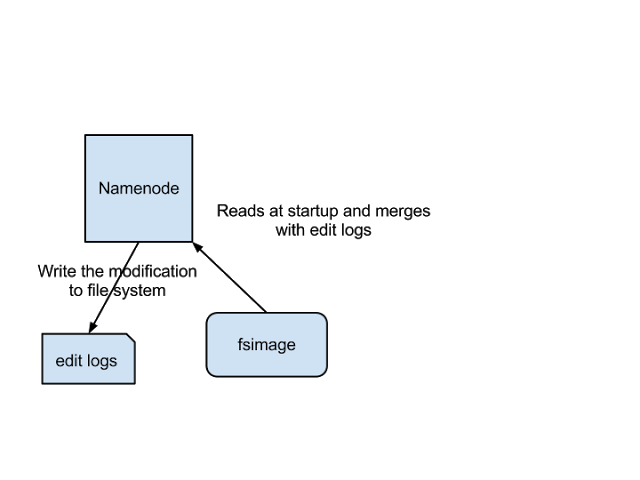
\includegraphics{images/namenode.png}
	\caption{NameNode}
	\label{img:grafik-nameNode}
\end{figure}

Wie aus der Abbildung zu sehen ist, schreibt ein NameNode zwei unterschiedliche Dateien auf die Festplatte. \\
\begin{itemsize}
\item FsImage ist eine Momentane Aufnahme des Dateisystem zum Zeitpunkt des Starts des NameNodes
\item Edit Logs beinhaltet eine Menge der Änderungen, die nach dem Starten eines NameNodes auftreten.
\end{itemsize}
Ein FsImage wird nur beim Neustart eines NameNodes geschrieben. Dabei wird die Information aus dem EditLog in den FsLog geschrieben um die momentane Aufnahme des Dateisystems zu speichern.\\
Da in der Regel ein NameNode sehr selten neu gestartet wird, entstehen folgende Probleme:
\begin{itemsize}
\item EditLog wird sehr groß und kann nicht verwaltet werden.
\item Das Neustarten eines NameNode dauert auf Grund der großen Datenmenge sehr lange.
\item Im Fall eines Ausfalls des NameNodes geht sehr große Menge an Information verloren.
\end{itemsize}
Secondary NameNode wird dafür benötigt um die oben beschriebenen Probleme zu umgehen.\\
\begin{figure}
	\centering
	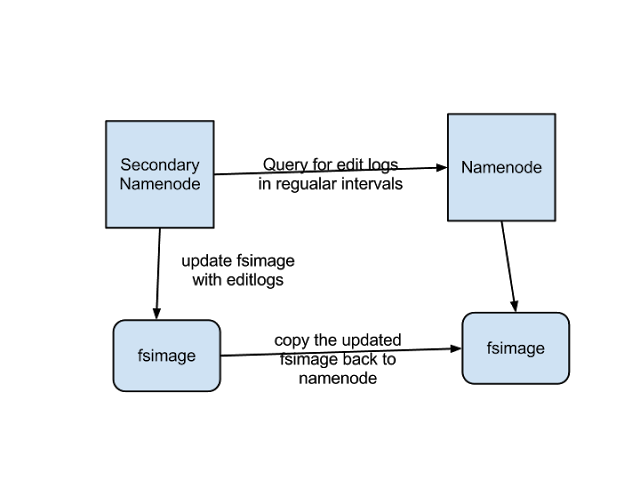
\includegraphics{images/secondarynamenode.png}
	\caption{SecondaryNameNode}
	\label{img:grafik-SecondaryNameNode}
\end{figure}
Aufgaben eines Secondary NameNodes sind:
\begin{itemsize}
\item Ein Secondary NameNode holt in der regelmäßigen Abständen die Daten aus dem EditLog und verschiebt sie in den FsImage.
\item Sobald ein neuer FsImage vorhanden ist, wird es auf den NameNode geschrieben.
\item 3. Der neue FsImage wird beim nächsten Neustart des NameNodes verwendet, was die Zeit des Prozess stark reduziert.
\end{itemsize}
[S1]
